\documentclass[letterpaper,headings=standardclasses]{scrartcl}

\usepackage[margin=1in,includefoot]{geometry}
\usepackage{amssymb}
\usepackage{amsmath}
\usepackage{listings}
\usepackage{tikz}
\usepackage{float}

\usetikzlibrary{shapes,arrows}

\tikzset{
  block/.style    = {draw, thick, rectangle, minimum height = 3em, minimum width = 3em},
  sum/.style      = {draw, circle},
  input/.style    = {coordinate, circle},
  output/.style   = {coordinate, circle}
}

\lstset{basicstyle=\ttfamily,language=python,columns=flexible,breaklines=true}

\title{Homework 1}
\subtitle{CS 559 - Neural Networks - Fall 2019}
\author{Matteo Corain 650088272}

\begin{document}

\maketitle

\section{Question 1}

\subsection{Logical products}

For the implementation of a logical product in a perceptron using the signum activation function, it is possible to derive a simple rule that, slightly modifying the one presented for perceptrons using step activation, allows to determine a possible set of weights that satisfies the given relationship. Let $f(x_1, \dots, x_n, x_{n+1}, \dots, x_{n+m})$ be a logical product in the form:

$$ f(x_1, \dots, x_n, x_{n+1}, \dots, x_{n+m}) = \bar{x_1} \dots \bar{x_n} x_{n+1} \dots x_{n+m} $$

When implemented in a perceptron using value $-1$ to represent a logical false, the following relation holds:

$$ f(x_1, \dots, x_n, x_{n+1}, \dots, x_{n+m}) = 1 \Leftrightarrow \begin{cases} x_1 = \dots = x_n = -1 \\ x_{n+1} = \dots = x_{n+m} = 1\end{cases}$$

Given that the signum activation function returns $1$ if and only if its argument is strictly positive, the above condition can be rewritten as follows:

$$ y = 1 \Rightarrow \text{sgn} \left( \sum_{i=0}^{n+m} w_i x_i \right) = 1 \text{ when } \begin{cases} x_1 = \dots = x_n = -1 \\ x_{n+1} = \dots = x_{n+m} = 1\end{cases} \Rightarrow$$

$$ \Rightarrow w_0 - \sum_{i = 0}^{n} w_i + \sum_{i = n+1}^{n+m} w_i > 0 $$

In analogy to what has been shown for perceptrons using the step activation function, let us associate each negated variable with a weight of $-1$ and each non-negated variable with a weight of $+1$. Using this convention, the value of $w_0$ should be such that is satisfies the previous relation:

$$ w_0 - \sum_{i = 0}^{n} (-1) + \sum_{i = n+1}^{n+m} (+1) > 0 \Rightarrow w_0 + n + m > 0 \Rightarrow w_0 > - n - m $$

At the same time, the bias $w_0$ must be such that, when at least an input is not in the requested logic state, then the output of the perceptron should go to a logical false ($-1$), which means the induced field of the neuron must be negative. In this case, given that false values are represented by $-1$, if a variable is in the wrong state, then the induced field of the neuron is decreased by $2$ (not only we do not count a $+1$, but we also have to account for a $-1$); this means that the following relationship should hold as well:

$$ w_0 + n + m - 2 < 0 \Rightarrow w_0 < - n - m  + 2$$

A good choice for the value of $w_0$ could therefore be:

$$ w_0 = - n - m + 1 $$

Using the presented rule, it is immediate to find a possible set of weights for a perceptron that implements the requested logical products. Let us start considering the first product $\bar{x_1} x_2 x_3$; in this case, we have $n=1$ complemented inputs ($x_1$) and $m=2$ non-complemented inputs ($x_2$ and $x_3$); therefore, a possible set of weights that implements this logic product is:

$$ w_0 = -1 -2 + 1 = -2 $$
$$ w_1 = -1, w_2 = w_3 = 1 $$

As a proof of the validity of the selected values, it is possible to show that these weights satisfy the system of linear inequalities which can be derived from the truth table of the logical product.

\begin{table}[h]
\centering
\begin{tabular}{|c|c|c|c|c|c|}
\hline
$x_1$ & $x_2$ & $x_3$ & $y$ & Inequality & Proof \\ \hline
-1    & -1    & -1    & -1  & $w_0-w_1-w_2-w_3<0$ & $-2+1-1-1=-3<0$ \\ \hline
-1    & -1    & +1    & -1  & $w_0-w_1-w_2+w_3<0$ & $-2+1-1+1=-1<0$ \\ \hline
-1    & +1    & -1    & -1  & $w_0-w_1+w_2-w_3<0$ & $-2+1+1-1=-1<0$ \\ \hline
-1    & +1    & +1    & +1  & $w_0-w_1+w_2+w_3>0$ & $-2+1+1+1=+1>0$ \\ \hline
+1    & -1    & -1    & -1  & $w_0+w_1-w_2-w_3<0$ & $-2-1-1-1=-5<0$ \\ \hline
+1    & -1    & +1    & -1  & $w_0+w_1-w_2+w_3<0$ & $-2-1-1+1=-3<0$ \\ \hline
+1    & +1    & -1    & -1  & $w_0+w_1+w_2-w_3<0$ & $-2-1+1-1=-3<0$ \\ \hline
+1    & +1    & +1    & -1  & $w_0+w_1+w_2+w_3<0$ & $-2-1+1+1=-1<0$ \\ \hline
\end{tabular}
\caption{Truth table for the first logical product using signum activation}
\label{truth_prod1}
\end{table}

The same process can be followed also for the implementation of the second logical product $ x_1 \bar{x_2} $; in this case, we have $ n = 1 $ ($x_1$) and $ m = 1 $ ($x_2$). A possible choice of weights that implements the requested logical function is:

$$ w_0 = -1 -1 + 1 = -1 $$
$$ w_1 = 1, w_2 = -1, w_3 = 0 $$

Also in this case it is possible to show the validity of the selected values using the truth table and deriving the corresponding system of linear inequalities.

\begin{table}[h]
\centering
\begin{tabular}{|c|c|c|c|c|}
\hline
$x_1$ & $x_2$ & $y$ & Inequality & Proof \\ \hline
-1    & -1    & -1  & $w_0-w_1-w_2<0$ & $-1-1+1=-1<0$ \\ \hline
-1    & +1    & -1  & $w_0-w_1+w_2<0$ & $-1-1-1=-3<0$ \\ \hline
+1    & -1    & +1  & $w_0+w_1-w_2>0$ & $-1+1+1=+1>0$ \\ \hline
+1    & +1    & -1  & $w_0+w_1+w_2<0$ & $-1+1-1=-1<0$ \\ \hline
\end{tabular}
\caption{Truth table for the second logical product using signum activation}
\label{truth_prod2}
\end{table}

\subsection{OR logical function}

For the implementation of the OR logical function, a custom design has been necessary since the two neurons in the first layer output value $-1$ for a logical false. The single neuron in the second layer of the network has to implement the function described by the truth table shown in table \ref{truth_or}.

\begin{table}[h]
\centering
\begin{tabular}{|c|c|c|}
\hline
$x_1$ & $x_2$ & $y$ \\ \hline
-1    & -1    & -1  \\ \hline
-1    & 1     & 1   \\ \hline
1     & -1    & 1   \\ \hline
1     & 1     & 1   \\ \hline
\end{tabular}
\caption{Truth table for the OR logical function using signum activation}
\label{truth_or}
\end{table}

For the design of this neuron, a graphical procedure has been followed, based on the geometric interpretation of the perceptron. If we plot the four labeled data points on the $x_1$-$x_2$ plane, as shown in figure \ref{or_func}, we can see that the two output classes are linearly separable; thus, it is possible to identify a line that allows to separate them.

A possible separator, shown in figure, is described by the relation:

$$ 1 + x_1 + x_2 = 0 $$

From the equation of this separator, we obtain that a possible selection of weights that allow for the implementation of the required logic function is the following:

$$ w_0 = w_1 = w_2 = 1 $$

This may also be analytically verified by writing down the system of linear inequalities that describe this logical function; in fact, from the truth table we have that:

$$ \begin{cases} \text{sgn(} w_0 - w_1 - w_2 \text{)} = -1 \\ \text{sgn(} w_0 - w_1 + w_2 \text{)} = 1 \\ \text{sgn(} w_0 + w_1 - w_2 \text{)} = 1 \\ \text{sgn(} w_0 + w_1 + w_2 \text{)} = 1 \end{cases} \Rightarrow \begin{cases} w_0 - w_1 - w_2 < 0 \\ w_0 - w_1 + w_2 > 0 \\ w_0 + w_1 - w_2 > 0 \\ w_0 + w_1 + w_2 > 0 \end{cases} \Rightarrow \begin{cases} 1 - 1 - 1 = -1 < 0 \\ 1 - 1 + 1 = 1 > 0 \\ 1 + 1 - 1 = 1 > 0 \\ 1 + 1 + 1 = 3 > 0 \end{cases} $$

\begin{figure}[h]
\centering
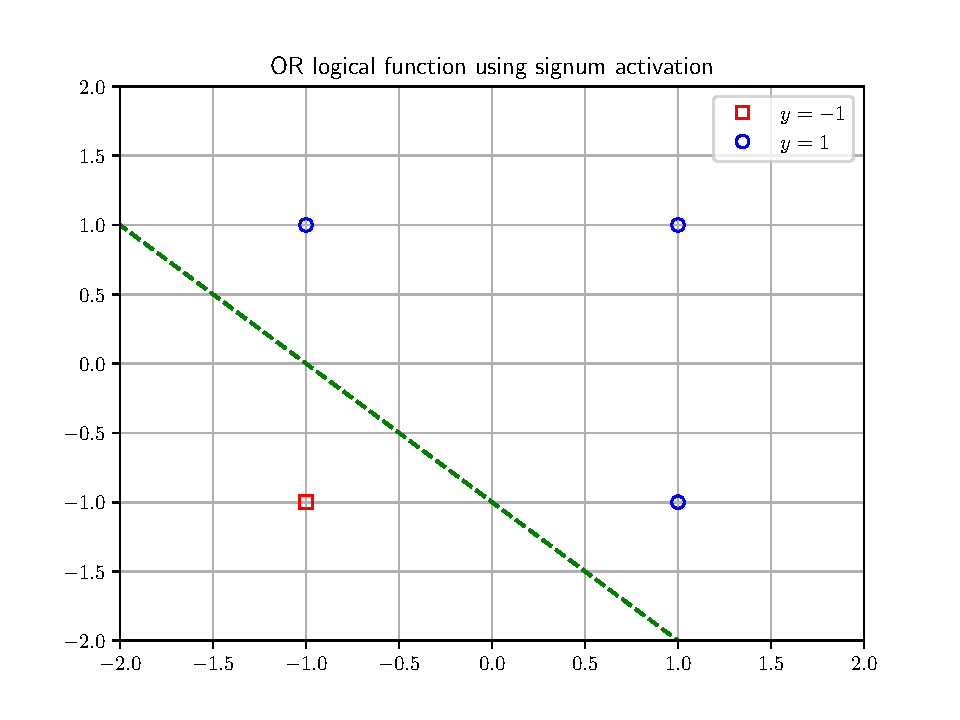
\includegraphics[width=.7\linewidth]{or_func.pdf}
\caption{Separator implementing the OR operator using signum activation}
\label{or_func}
\end{figure}

\subsection{Final network}

A possible network that implements the logical function $f(x_1,x_2,x_3) = \bar{x_1} x_2 x_3 + x_1 \bar{x_2}$, using the previously selected weights, is depicted in figure \ref{final_net}.

\begin{figure}[H]
\centering
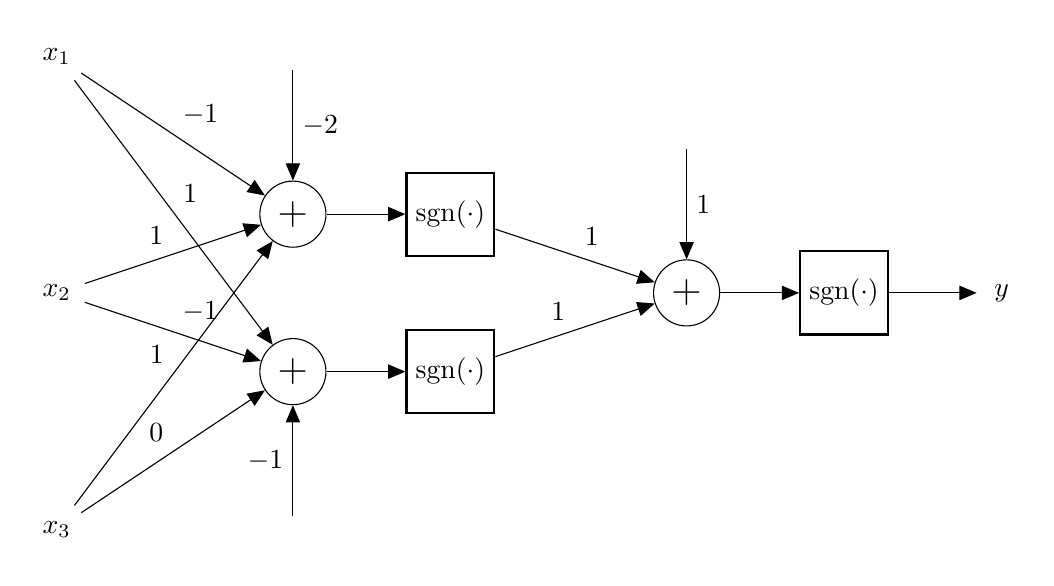
\begin{tikzpicture}[auto, node distance=2cm, >=triangle 45]

% Input layer
\draw node [input, name=x1] {$x_1$};
\draw node [input, name=x2, below of=x1, node distance=3cm] {$x_2$};
\draw node [input, name=x3, below of=x2, node distance=3cm] {$x_3$};

% First layer
\draw node [sum, right of=x2, yshift=1cm, node distance=3cm] (sum1) {\Large$+$};
\draw node [sum, below of=sum1] (sum2) {\Large$+$};
\draw node [input, name=x01, above of=sum1] {};
\draw node [input, name=x02, below of=sum2] {};
\draw node [block, right of=sum1] (act1) {sgn($\cdot$)};
\draw node [block, right of=sum2] (act2) {sgn($\cdot$)};

% Second layer
\draw node [sum, right of=act1, yshift=-1cm, node distance=3cm] (sum3) {\Large$+$};
\draw node [input, name=x03, above of=sum3] {};
\draw node [block, right of=sum3] (act3) {sgn($\cdot$)};
\draw node [output, name=y, right of=act3] {$y$};

% Connections
\draw[->](x01) -- node {$-2$}(sum1);
\draw[->](x1) -- node {$-1$}(sum1);
\draw[->](x2) -- node {$1$}(sum1);
\draw[->](x3) -- node {$1$}(sum1);
\draw[->](x02) -- node {$-1$}(sum2);
\draw[->](x1) -- node {$1$}(sum2);
\draw[->](x2) -- node {$-1$}(sum2);
\draw[->](x3) -- node {$0$}(sum2);
\draw[->](sum1) -- node {}(act1);
\draw[->](sum2) -- node {}(act2);
\draw[->](x03) -- node {$1$}(sum3);
\draw[->](act1) -- node {$1$}(sum3);
\draw[->](act2) -- node {$1$}(sum3);
\draw[->](sum3) -- node {}(act3);
\draw[->](act3) -- node {}(y);

\end{tikzpicture}
\caption{Final network that implements the given function}
\label{final_net}
\end{figure}

\section{Question 2}

\subsection{Analysis of the first layer}

In order to sketch the region in which the output of the network is $z = 1$, let's begin considering the first layer of neurons independently; for each of them, it is possible to write the input-output relationship, starting from the given weights:

\begin{itemize}

\item The first neuron implements the function $z_1 = u(1 + x - y)$, meaning that its output goes to 1 when $1 + x - y \ge 0 \Rightarrow y \le x + 1$;
\item The second neuron implements the function $z_2 = u(1 - x - y)$, meaning that its output goes to 1 when $1 - x - y \ge 0 \Rightarrow y \le -x + 1$;
\item The third neuron implements the function $z_3 = u(-x)$, meaning that its output goes to 1 when $-x \ge 0 \Rightarrow x \le 0$.

\end{itemize}

The regions in which the three neurons output a positive value can be represented on the $x$-$y$ plane as shown in the figure \ref{first_layer_out_sep}.

\begin{figure}[h]
\centering
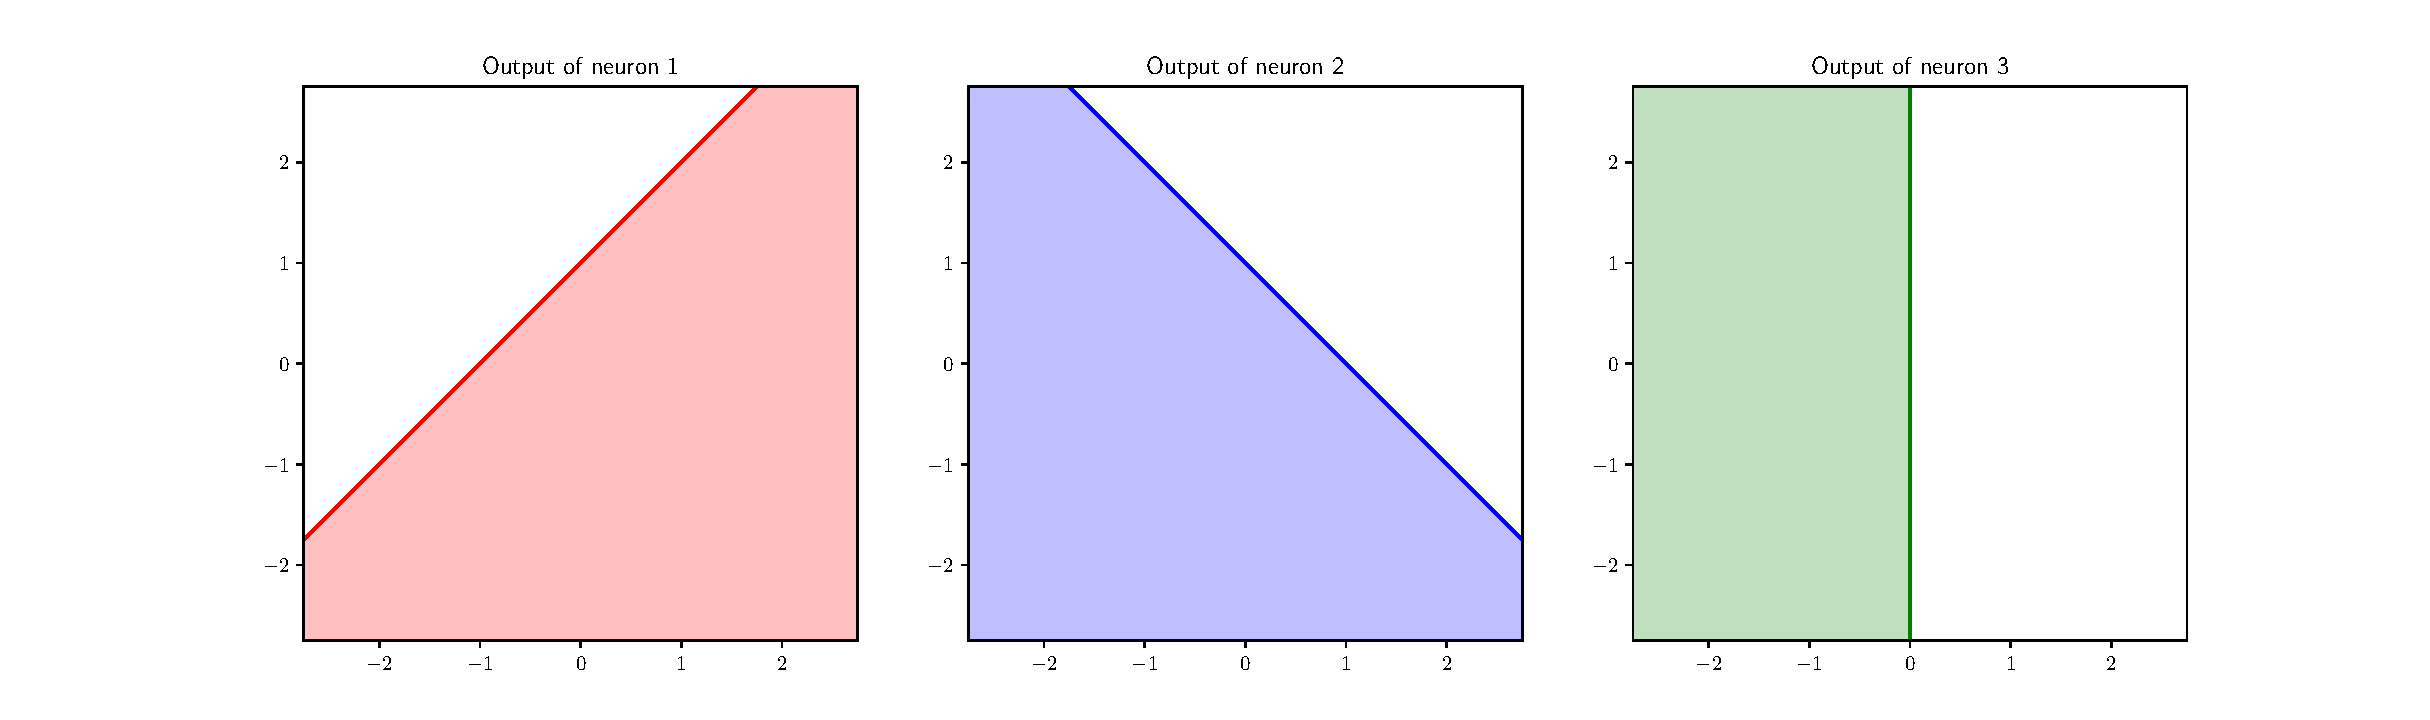
\includegraphics[width=\linewidth]{first_layer_out_sep.pdf}
\caption{Regions in which first layer neurons output a positive value}
\label{first_layer_out_sep}
\end{figure}

\subsection{Deduction of network output per region}

If we represent all those relationships on a single plane, then six different regions can be identified; each of those regions will represent a specific set of inputs of the second layer of the network. Analyzing those regions one by one, it is possible to deduce, for each of them, what will be the output of the network, given the input-output relationship of the second-layer neuron ($z = -1.5 + z_1 + z_2 - z_3$, where $z_1, z_2, z_3$ denote the outputs of the first-layer neurons):

\begin{figure}[h]
\centering
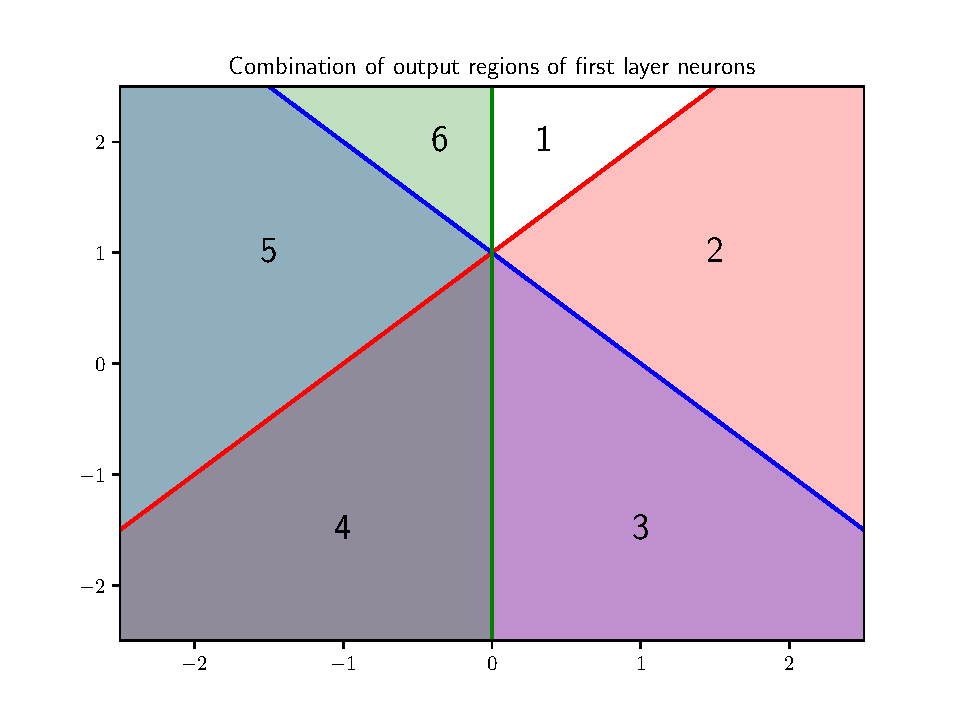
\includegraphics[width=0.7\linewidth]{first_layer_out_all.pdf}
\caption{Combination of output regions of first layer neurons}
\label{first_layer_out_all}
\end{figure}

\begin{enumerate}

\item In this region, the outputs of all first layer neurons is zero; therefore, the output $z$ of the neuron in the second layer is:

$$ z = u(-1.5 + 1 * 0 + 1 * 0 - 1 * 0) = u(-1.5) = 0 $$

\item In this region, the output of the first neuron is positive, while the outputs of the others are zero; therefore, the output $z$ of the neuron in the second layer is:

$$ z = u(-1.5 + 1 * 1 + 1 * 0 - 1 * 0) = u(-0.5) = 0 $$

\item In this region, the output of the first and second neurons are positive, while the output of the third is zero; therefore, the output $z$ of the neuron in the second layer is:

$$ z = u(-1.5 + 1 * 1 + 1 * 1 - 1 * 0) = u(0.5) = 1 $$

\item In this region, the outputs of all first layer neurons is positive; therefore, the output $z$ of the neuron in the second layer is:

$$ z = u(-1.5 + 1 * 1 + 1 * 1 - 1 * 1) = u(-0.5) = 0 $$

\item In this region, the output of the second and third neurons are positive, while the output of the first is zero; therefore, the output $z$ of the neuron in the second layer is:

$$ z = u(-1.5 + 1 * 0 + 1 * 1 - 1 * 1) = u(-1.5) = 0 $$

\item In this region, the output of the third neuron is positive, while the outputs of the others are zero; therefore, the output $z$ of the neuron in the second layer is:

$$ z = u(-1.5 + 1 * 0 + 1 * 0 - 1 * 1) = u(-2.5) = 0 $$

\end{enumerate}

The only region in which the network returns a positive value, therefore, is region number 3, including the separator of the second neuron (the blue line, on which the second neuron outputs $u(0) = 1$) but excluding the one of the third neuron (the green line, on which the third neuron outputs $u(0) = 1$). Graphically, it is possible to represent the two classes separated by this network on the $x$-$y$ plane as shown in figure \ref{net_sep}; the dashed line indicates a zone for which $z = 0$, while the normal line a zone for which $z = 1$.

\begin{figure}[h]
\centering
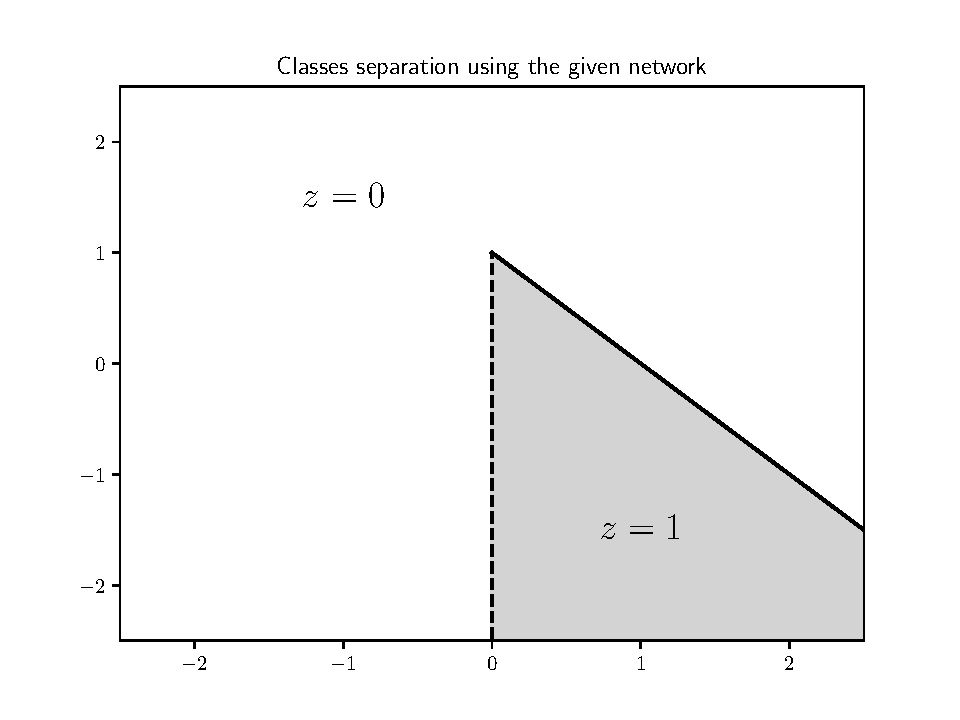
\includegraphics[width=0.7\linewidth]{net_sep.pdf}
\caption{Classes separation using the given network}
\label{net_sep}
\end{figure}

\section{Question 3}

\subsection{Exact weights selection}

The first step of the problem require to generate a random vector of exact weights, which will be used later for the classification of the training samples. This has been accomplished by means of the \texttt{uniform()} function in the \texttt{random} package of the NumPy library (the adopted programming language is Python); the generated weights have then been used to construct a Numpy array named $w_r$. To guarantee the reproducibility of the results, all values have been generated after having fixed the seed of the random generator, in this case to 10. The obtained weights are then logged to the console; for this particular instance of the script, they were picked as:

$$ w_r = [\begin{matrix} 0.135660320 & -0.9584961 & 0.26729647 \end{matrix}] $$

\subsection{Generation of the training set}

The same approach has been used for the generation of the training set $\mathcal{S}$ for the network. This has been populated using the list comprehension syntax provided by the Python language, which allows to repeat the same action (in this case, the creation of a NumPy array having two randomly picked components) for a given number of times, described by the variable $n$ (set to 100). For convenience and efficiency, the training samples have been generated with an additional first component identically set to 1: this allows to multiply those vectors directly with a weights vector, taking into consideration also the contribution given by the perceptron's bias.

After the generation of the training set, the samples have been classified in two groups, $\mathcal{S}_0$ and $\mathcal{S}_1$, according to the output returned by an “ideal” perceptron using the computed exact weights. For this purpose, the list comprehension syntax has been used again; in a first step, the vector of the desired outputs $d$ has been computed, whose components are set to 1 in the case the result of the product $[ \begin{matrix}1 & x_1 & x_2 \end{matrix}][\begin{matrix} w_0 & w_1 & w_2 \end{matrix}]^T$ is positive, 0 otherwise. Using these data, the two sets $\mathcal{S}_0$ and $\mathcal{S}_1$ may be simply computed by considering the elements of the training set $x_i \in \mathcal{S}$ having respectively $d_i = 0$ or $d_i = 1$. For this particular instance of the script, we had 43 samples in set $\mathcal{S}_0$ and 57 in set $\mathcal{S}_1$.

\subsection{Plotting data and separator}

\begin{figure}[h]
\centering
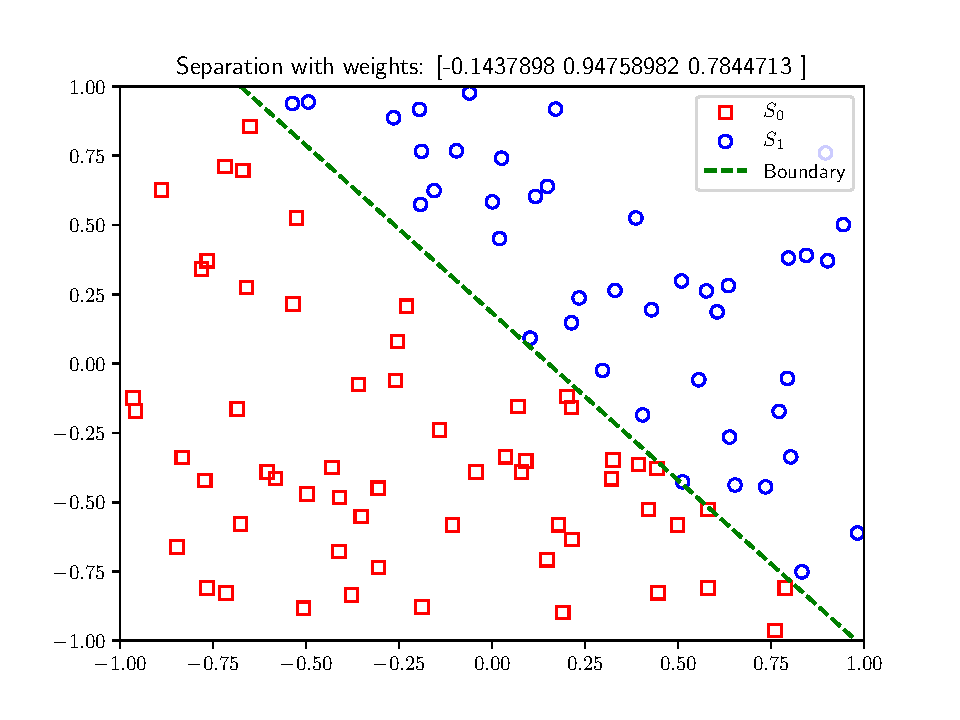
\includegraphics[width=.7\linewidth]{exact_sep.pdf}
\caption{Data separation using the exact weights}
\label{exact_sep}
\end{figure}

In order to plot the data and the ideal separator on the $x_1$-$x_2$ plane, the \texttt{plot\_data\_and\_sep()} function has been defined. This takes as parameters the two sets $\mathcal{S}_0$ and $\mathcal{S}_1$, and the vector of weights $w$ to be used. The function performs the following actions:

\begin{itemize}

\item It initializes a new Matplotlib figure;

\item It plots a data point, represented as a blue square, for each element in set $\mathcal{S}_0$, using as its $x$ value its second component (the first is identically set to 1) and as its $y$ value its third component;

\item It plots a data point for each element in $\mathcal{S}_1$, represented as an orange circle;

\item It plots the separator line in dashed green, using as $x$ values -1 and 1 and as $y$ values the ones computed by expliciting the linear relationship for $x_2$ and substituting $x_1$ with -1 and 1:

$$ x_2 = -\frac{w_0 + w_1 x_1}{w_2} $$

\item It sets the boundaries of the figure to $[-1;1]$ along both axes;

\item It prints a title and a legend, then shows the result without blocking the execution.

\end{itemize}

The resulting separation for this particular instance of the script is shown in figure \ref{exact_sep}.

\subsection{Running the Perceptron Training Algorithm}

The Perceptron Training Algorithm has been coded as a separate function, called \texttt{pta()}, which takes as argument the value of the parameter $\eta$ to be used, the vector $w_0$ of initial weights, the training set $\mathcal{S}$ and the vector of the desired outputs $d$. This function implements a slightly modified version of the standard PTA, performing the following actions:

\begin{itemize}

\item It initializes the PTA variables, creating a copy $w$ of the array $w_0$ that will be used to compute the final weights and setting to 0 the number of $epochs$ of the algorithm;

\item It initializes a list, called $mclass$, in which the number of misclassified objects is stored for each epoch (starting from epoch 0, which is the number of misclassifications when the initial random weights are used); those are computed using the \texttt{count\_mclass()} function, which performs the inline sum of the elements of a vector (created using the list comprehension syntax) whose components are set to 1 in case the value of the product $wx^T$ is different to the expected one, stored in the vector $d$;

\item It starts a \texttt{while} loop, which stops when the number of misclassification at the previous epoch has reached zero (we have found the weights that correctly classify the entire training set); at each iteration:

\begin{itemize}

\item It increments the number of $epochs$;

\item It loops through all training samples $x_i$, updating the weights according to the formula:

$$ w = w + \eta x_i (d_i - u(w x_i)) $$

\item It computes the number of misclassifications for the current epoch and logs the results.

\end{itemize}

\item When the loop terminates, the procedure returns the array of the computed weights $w$, the number of $epochs$ and the list of misclassifications per epoch $mclass$.

\end{itemize}

This function is made run multiple times with a variable value of $\eta$ but with a fixed initial vector $w_0$, so that the differences in the results depend only on the selected value of the parameter. For this particular instance of the script, the initial random vector of weights has been chosen as:

$$ w' = [\begin{matrix} 0.72895839 & -0.23193846 & -0.48539423 \end{matrix}] $$

The obtained weights with the corresponding number of epochs needed for their computation are shown in the table below.

\begin{table}[h]
\centering
\begin{tabular}{|c|c|c|c|c|}
\hline
$\eta$ & $w_0$       & $w_1$        & $w_2$       & Epochs \\ \hline
1      & 0.72895839  & -5.28189517  & 1.07831069  & 7      \\ \hline
10     & 10.72895839 & -73.141983   & 27.11808154 & 26     \\ \hline
0.1    & 0.12895839  & -0.88238499  & 0.2929104   & 33     \\ \hline
\end{tabular}
\caption{Computed weights using different values of $\eta$}
\end{table}

\subsection{Considerations on the computed weights}

At a first sight, the weights returned by the algorithm running with the different values of $\eta$ seem very different with respect to the “exact” ones, and so it should be since the parameter $\eta$ appears as a multiplication factor in the different steps of the agorithm. Using greater values of $\eta$ yields greater weights (in absolute terms), while using smaller values of the parameter yields smaller weights (in absolute terms), since at each step the weights are updated by summing a quantity equal to $\eta x_i (d_i - u(w x_i))$.

In fact, the value of the computed weights is not meaningful in absolute terms. In order to understand what kind of relation holds between the computed and the exact weights, we have to recall the equation of the linear separator that a perceptron implements:

$$ w_0 + w_1x_1 + w_2x_2 = 0 $$

To give this equation a geometric interpretation, let us rewrite it in a more usual form, expliciting the value of the variable $x_2$ in terms of the variable $x_1$:

$$ x_2 = -\frac{w_1x_1 + w_0}{w_2} = -\frac{w_1}{w_2}x_1 -\frac{w_0}{w_2} $$

This is indeed the equation of a line in the $x_1$-$x_2$ plane, having:

$$ m = -\frac{w_1}{w_2}, q = -\frac{w_0}{w_2} $$

The $m$ and $q$ parameters are, in this case, the real values of interest, since they allow to characterize the separator in an unambiguous way, regardless of the order of magnitude of the weights computed by the algorithm. If we calculate the values of $m$ and $q$ for all the set of weights, we obtain the result in table \ref{m_q_weights}.

\begin{table}[h]
\centering
\begin{tabular}{|c|c|c|}
\hline
$\eta$ & $m$ & $q$ \\ \hline
Exact  & $3.585891$ & $-0.50753$ \\ \hline
1      & $4.898306$ & $-0.67602$ \\ \hline
10     & $2.697166$ & $-0.39564$ \\ \hline
0.1    & $3.012474$ & $-0.44027$ \\ \hline
\end{tabular}
\caption{Values of $m$ and $q$ for each set of weights}
\label{m_q_weights}
\end{table}

As it can be seen, the values computed for the obtained weights are actually comparable to the ones computed for the exact ones, which means that the algorithm has been able to converge to a set of lines that are all able to separate the two classes of data, as shown in figure \ref{all_sep} (obtained using function \texttt{plot\_data\_and\_sep\_all()}, a variation of \texttt{plot\_data\_and\_sep()}).

\begin{figure}[h]
\centering
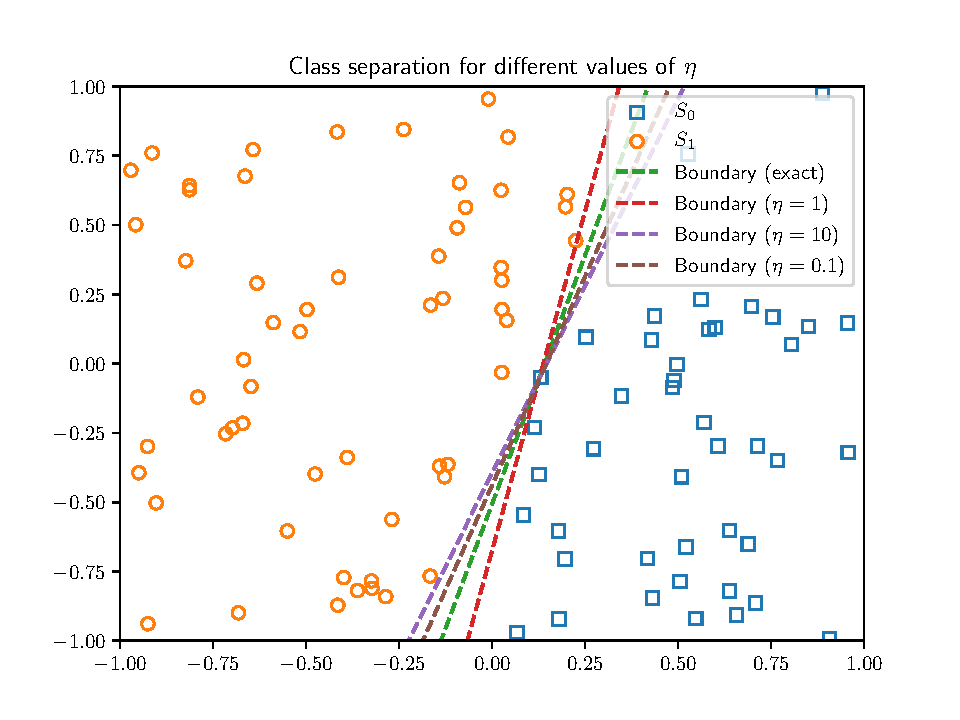
\includegraphics[width=0.7\linewidth]{all_sep.pdf}
\caption{Separation obtained using the computed sets of weights}
\label{all_sep}
\end{figure}

The correspondence between the values of $m$ and $q$ would have been even better if we had a greater number of data points placed very near to the separator itself. In this case, in fact, a greater precision would have been requested to the perceptron to separate the two classes; to achieve that, the algorithm would have needed to update the obtained weights in a way that the $m$ and $q$ parameter would have been closer to the expected ones.

If we considered a perceptron with more than two inputs, this approach may be easily generalized; in this case, the linear equation of the separator describes a hyperplane and has the generic form:

$$ w_0 + w_1x_1 + \dots + w_{n-1}x_{n-1} + w_nx_n = 0 $$

Using an analogous procedure, let us explicit the value of $x_n$ from this relationship, obtaining:

$$ x_n = -\frac{w_0}{w_n} - \frac{w_1}{w_n}x_1 - \dots \frac{w_{n-1}}{w_n}x_{n-1} = - k_0 - k_1x_1 - \dots - k_{n-1}x_{n-1} $$

The parameters $k_0 \dots k_{n-1}$ of this linear equation are, in this case, the values of interest, that make the results obtained by different runs of the algorithm comparable.

\subsection{Plotting the misclassification rate}

\begin{figure}[h]
\centering
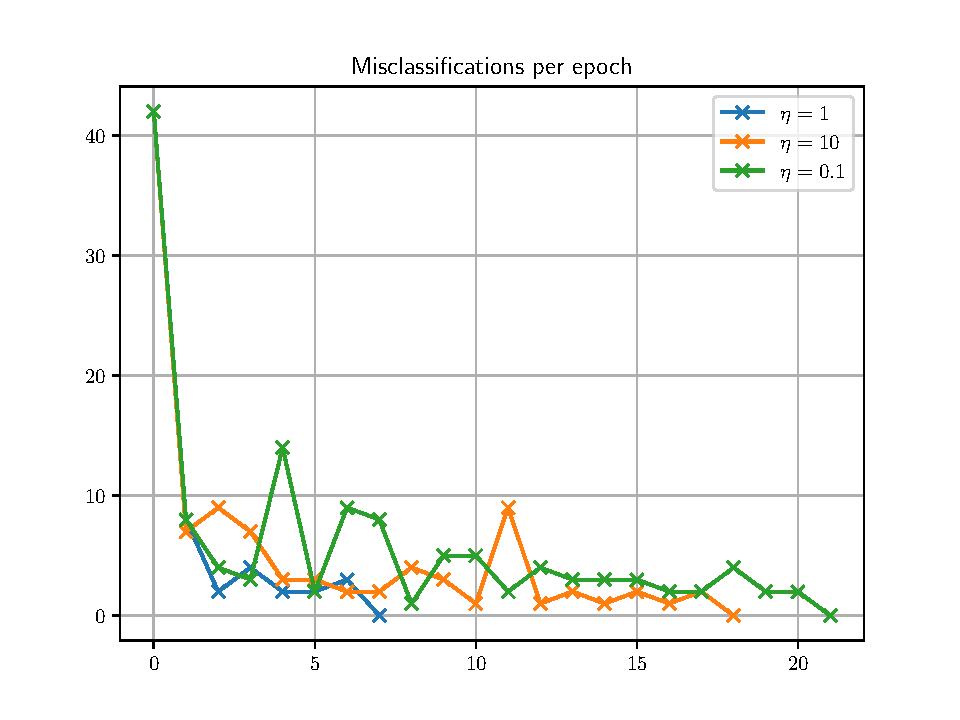
\includegraphics[width=.7\linewidth]{mclass_per_epoch.pdf}
\caption{Number of misclassified items per epoch}
\label{mclass_per_epoch}
\end{figure}

After each run of the algorithm, the number of misclassified objects per epoch is plotted by means of the \texttt{plot\_mclass()} function; this performs the following actions:

\begin{itemize}

\item It initializes a new Matplotlib figure;

\item It plots the number of misclassification against the number of the epoch for each value of the parameter $\eta$ (epoch 0 represents the initial number of misclassified objects, computed using the random weights);

\item It prints a title and a legend for the graph, enables the grid and shows the result without blocking the execution.

\end{itemize}

As shown in figure \ref{mclass_per_epoch}, the number of misclassifications decreases as expected with the epoch number, although not always monotonically; it finally reaches zero when the desired weights have been computed.

\subsection{Effects of the value of $\eta$ on convergence speed}

The selection of the $\eta$ parameter of the Perceptron Training Algorithm affects the convergence speed of the algorithm in two ways:

\begin{itemize}

\item If it is too low, then the algorithm may require a larger number of epochs to converge since the weights are updated by summing a more limited quantity at each epoch;

\item If it is too high, then the algotithm may also require a larger number of epochs since the misclassification rate may present oscillations due to the significant update of the weights.

\end{itemize}

In this specific execution scenario, the value which turned out to be the best overall in terms of epochs to reach convergence was $\eta = 1$ (7 epochs), while both $\eta = 10$ and $\eta = 0.1$ required more (26 and 33 epochs, respectively).

From the plot of the number of misclassifications per epoch, it is possible to notice how the smaller update rate when $\eta = 0.1$ helped to prevent the spike in the misclassification rate at epoch 2, but on the other side caused the algorithm to take longer to converge. At the same time, the long number of epochs in which the run with $\eta = 10$ stabilized to a single misclassification can be motivated by the presence of data points close enough to the ideal separator such that, each time the weights were updated, a single one was always misclassified.

Those results are absolutely specific to this selection of the exact weights, of the training data set and of the initial weights for the algorithm. In particular:

\begin{itemize}

\item If we chose a different set of exact weights keeping constant the other parameters, a different separator would have been used; starting from the same initial weights, the algorithm would have needed to modify them in a more or less pronounced way, requiring either a bigger or smaller $\eta$ for the convergence in the lowest number of epochs;

\item If we chose a different training set keeping constant the other parameters, the distribution of data in the two classes would have changed; this means that the algorithm would have been able to find different combinations of weights which are able to separate them, requiring different values of $\eta$ for the fastest convergence;

\item If we chose a different set of initial weights keeping constant the other parameters, again the algorithm would have needed to modify them in a more or less pronounced way to reach a suitable solution, requiring different values of $\eta$ for the fastest convergence.

\end{itemize}

\subsection{Differences given by a larger number of samples}

If we repeat the previous operations using a larger number of samples ($n$ set to 1000), we can observe a few changes with respect to the run of the algorithm using only 100 samples. Table \ref{results_1000} sums up the results obtained in this second run of the algorithm.

\begin{table}[h]
\centering
\begin{tabular}{|c|c|c|c|c|c|c|}
\hline
$\eta$ & $w_0$ & $w_1$ & $w_2$ & $m$ & $q$ & Epochs \\ \hline
Exact & $0.13566032$ & $-0.9584961$ & $0.26729647$ & $3.585891$ & $-0.50753$ & \\ \hline
1 & $1.37044601$ & $-9.87497359$ & $2.71094556$ & $3.642631$ & $-0.50552$ & 5 \\ \hline
10 & $19.37044601$ & $-145.49718949$ & $38.69207426$ & $3.760387$ & $-0.500631$ & 18 \\ \hline
0.1 & $0.27044601$ & $-1.88394619$ & $0.53153825$ & $3.544329$ & $-0.508799$ & 38 \\ \hline
\end{tabular}
\caption{Results for the second run of the algorithm (1000 samples)}
\label{results_1000}
\end{table}

In particular, we can observe two facts:

\begin{itemize}

\item The values for $m$ and $q$ obtained from the computed weights are closer to the ones obtained from the exact weights;

\item The number of epochs required for convergence varies.

\end{itemize}

The first fact may be motivated since, due to growth of the training set, statistically a larger number of samples is distributed in close proximity to the exact separator. In order to find a line that can separate those data points, the algorithm needs to be more “precise” in determining (indirectly, through the computation of the weights) the values of the $m$ and $q$ parameters to be used. Figure \ref{all_sep_1000} shows the computed separators on the $x_1$-$x_2$ plane; it is possible to notice how the different lines are now much closer to the exact separator.

\begin{figure}[h]
\centering
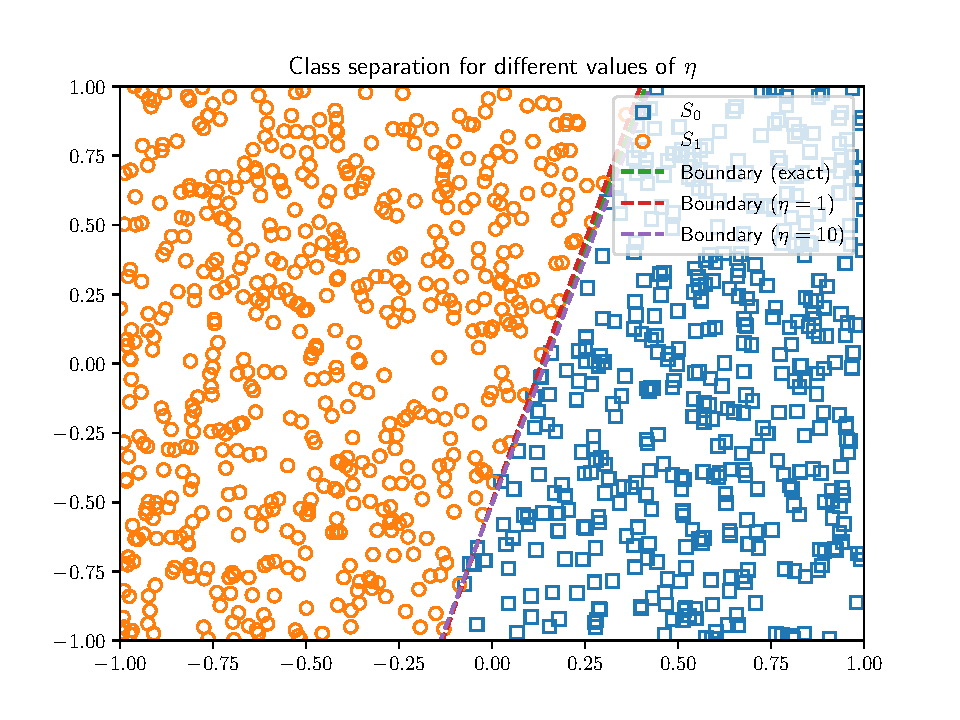
\includegraphics[width=0.7\linewidth]{all_sep_1000.pdf}
\caption{Separation obtained using the computed sets of weights (1000 samples)}
\label{all_sep_1000}
\end{figure}

The usage of a different data set impacts, as already explained, also on the optimal value of $\eta$ to be used. Similarly to the previous case, the best convergence time has been obtained using $\eta = 1$; both cases with $\eta = 1$ and $\eta = 10$ reached convergence in a lower number of epochs with respect to the previous case (this may be due to the greater number of samples, which make possible to update the computed weights a greater number of times for each epoch), while the case with $\eta = 0.1$ required more epochs than in the previous case. Figure \ref{mclass_per_epoch_1000} shows the misclassification rate per epoch for the three values of $\eta$.

\begin{figure}[h]
\centering
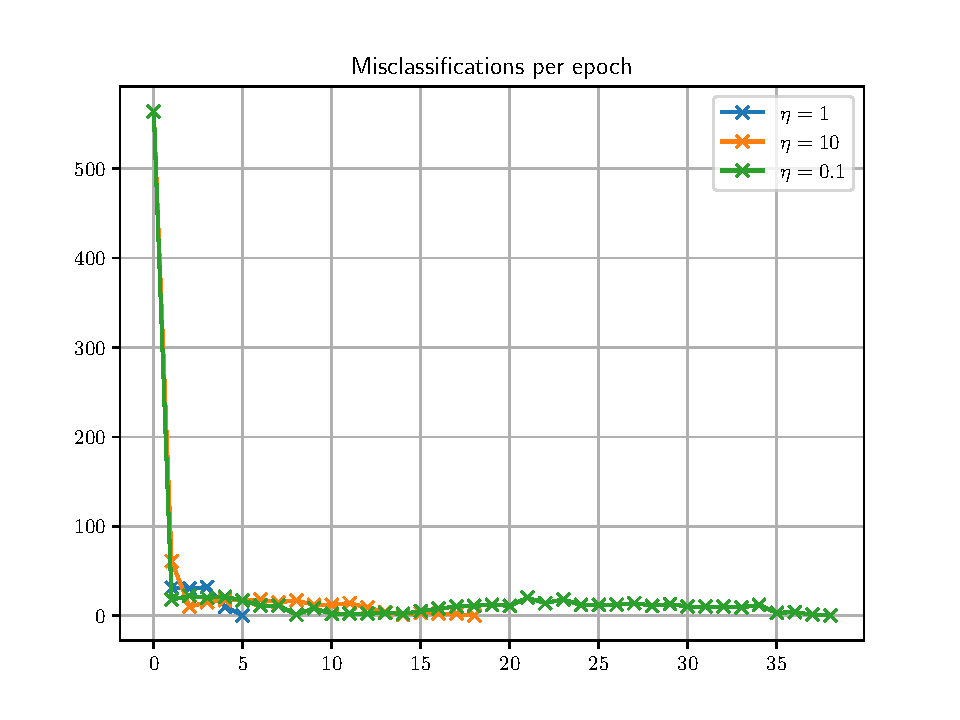
\includegraphics[width=.7\linewidth]{mclass_per_epoch_1000.pdf}
\caption{Number of misclassified items per epoch (1000 samples)}
\label{mclass_per_epoch_1000}
\end{figure}

\subsection{Complete Python code}

\lstinputlisting[basicstyle=\ttfamily\scriptsize]{hw1_ex3.py}

\end{document}